\chapter[Generacion procedural de contenidos]{\label{identificadorReferenciaCruzada}
Generacion procedural de contenidos}

La generación procedural de contenidos, se refiere a la creación de contenido del juego automáticamente, hay distintos aspectos que se pueden hacer con esta generación de contenidos:

\begin{itemize}
	\item Actuaciones de NPC
	\item Mapas y niveles
	\item Historias y diálogos
	\item Misiones
	\item Armas
	\item Personajes
\end{itemize}


Como se ha mencionado anteriormente, nos centraremos en la creación de contenido procedural de mapas y niveles, concretamente el proyecto irá centrado en la creación de mundos en 2D con ciudades que podrán verse en 3D al acercarte a estas.

Hay varias distinciones que hay que realizar para la generación de contenidos:

\begin{itemize}

\item una de las más importantes, es si el juego es online u offline.

\item Debemos de comprobar si el contenido generado es opcional o es necesario para el juego, ya que si es necesario debemos realizar algoritmos con mayor optimización que si es un contenido opcional.

\item Debemos tener en cuenta la utilización de  semillas aleatorias o de vectores con parámetros, ya que de ello dependerá el tipo de generación que queramos obtener.

\item La elección de una generación estocástica o determinística dependerá de si queremos que el algoritmo nos genere una misma solución con distintos parámetros.

\item Debemos de tener en cuenta si queremos generar de forma constructiva o generar y hacer un test en el que se mostraría la validez del resultado.

\end{itemize}

\section{Algoritmos de generación de contenido procedural:}

Estos algoritmos se bansan en la idea de generación y test de para generación procedural de contenidos, siendo el test es una función que acepta o rechaza el candidato y esto se almacena en un vector denominado fitness y también cuenta con un valor que se le ha asignado al nuevo candidato  al generarse, como puede verse en la figura \ref{Figura1}.\cite{B3}

\begin{figure}[h!]

	\centering
	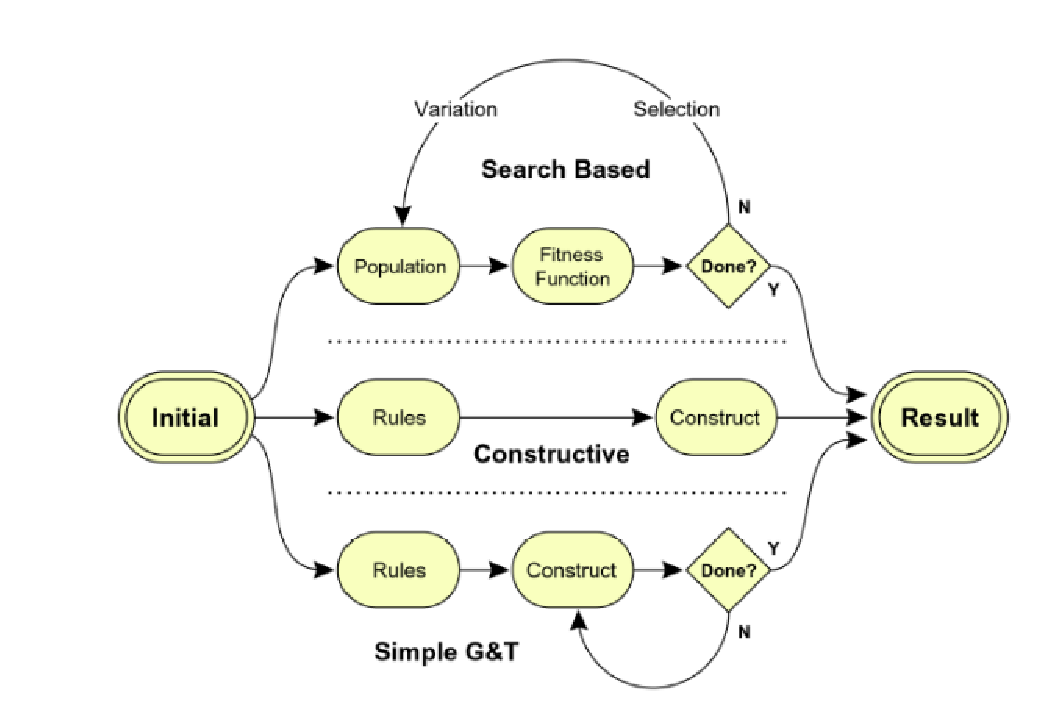
\includegraphics[width=9cm]{./eps/fig1.eps}
	\caption{Generación de reglas, extraído de \cite{B3}}
	\label{Figura1}

\end{figure}


Para la generación procedural son necesarias unas reglas que vayan asociadas a las mecánicas de juego, por ejemplo:\cite{B3}
\begin{itemize}
\item{\bf Hom and Marks} generaron unas reglas que eran representadas en el juego y estaban basadas en una función de evaluación de simulación estática y la teoría impulsada.

\item{\bf Browne} creó un sistema de diseño de reglas para direccionamiento usando programación genética, las reglas del juego estaban representadas en árboles, el lenguaje fue formulado para el proyecto.

\end{itemize}

\newpage
En la figura \ref{Figura2} podemos ver como se generan las reglas del juego:

\begin{figure}[h!]

	\centering
	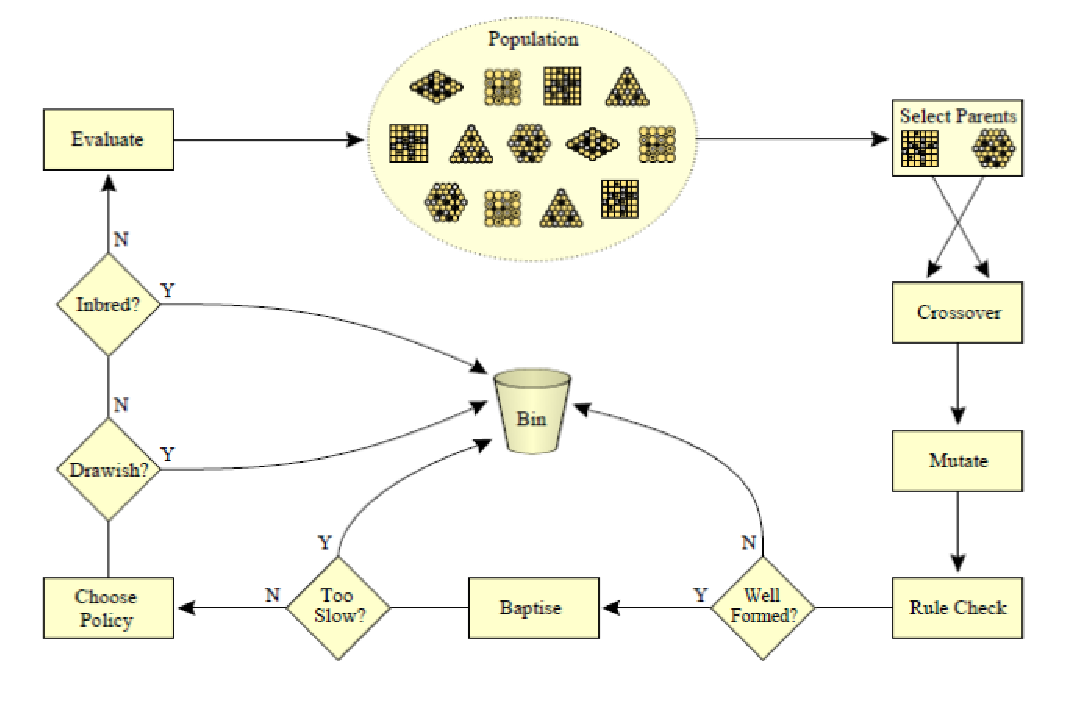
\includegraphics[width=9cm]{./eps/fig2.eps}
	\caption{Generación de reglas, extraído de \cite{B3}}
	\label{Figura2}

\end{figure}

\section{Representación del espacio de búsqueda:}

Una distinción importante en la representación es entre la codificación directa o indirecta ya que una codificación directa implica una relativa simpleza computacional en el mapeo del genotipo-fenotipo, dado que en una computación compleja es necesario la creación del fenotipo desde el genotipo.\cite{B6}\cite{B7}

En nuestro caso, una forma de representar el terreno es en forma de expresiones de árboles.


\section{Funciones de evaluación:}	

La evaluación es importante para ver las capacidades del algoritmo, para confirmar con garantía lo que puede crear y para comparar el contenido generado con otros contenidos.


Para diseñar la función de evaluación el diseñador debe primero decidir cuánto quiere optimizar para fortalecer el diseño.\cite{B8}


Tres tipos de evaluación son:

\begin{itemize}

\item Evaluación directa por funciones: en la que directamente una función saca el valor del fitness del contenido generado.

\item Evaluación simulada por funciones: en el que el contenido se va manipulando y se va evaluando.


\item Evaluación interactiva: mientras el juego está en ejecución se evalúa la interacción con el personaje y se van generando los contenidos.

\end{itemize}

Respecto a nuestro problema si realizamos una evaluación en cada punto que se determina mediante la consulta de árboles de expresión  que van evolucionando y sustitimos las coordenadas de la posición actual por coordenadas de las constantes del árbol, tendríamos una buena evaluación para la generación de mapas, esta forma está basada en la {\bf teoría de accesibilidad} en la cual se evalúa el terreno en función de la pendiente.

Para elegir las métricas apropiadas para la medición de la construcción es necesario esforzarse en la elección de medidas lo más lejanas posibles de los parámetros de entrada al sistema.





